\chapter{A kiberbiztonsági analízis megvalósítása}
% Technikai leírása a modellező eszköz architektúrájának
A következő fejezetnek a célja, hogy bemutassa az előző fejezetek által körülírt metodológia végrehajtását segítő fenyegetésmodellező eszközt, valamint a rendszermodellek származtatására készített szkriptet.

Az első alfejezetben látható egy áttekintés majd két fő részre osztva láthatóak a további alfejezetek. A két fő rész egyike a rendszerből kiberbiztonsági modell transzformálást mutatja be és az ezt segítő eszközöket. A másik pedig az EMF alapon implementált modellező eszközt amely a kiberbiztonsági modell alapján képes a manuális analízist támogatni dokumentumok generálásával valamint a támadási fák szerkesztésével.

\section{Áttekintés}

Egy áttekintése az elemző eszköz részeinek megtekinthető a \ref{fig:04_OVERVIEW} ábrán.

\begin{figure}[!ht]
	\centering
	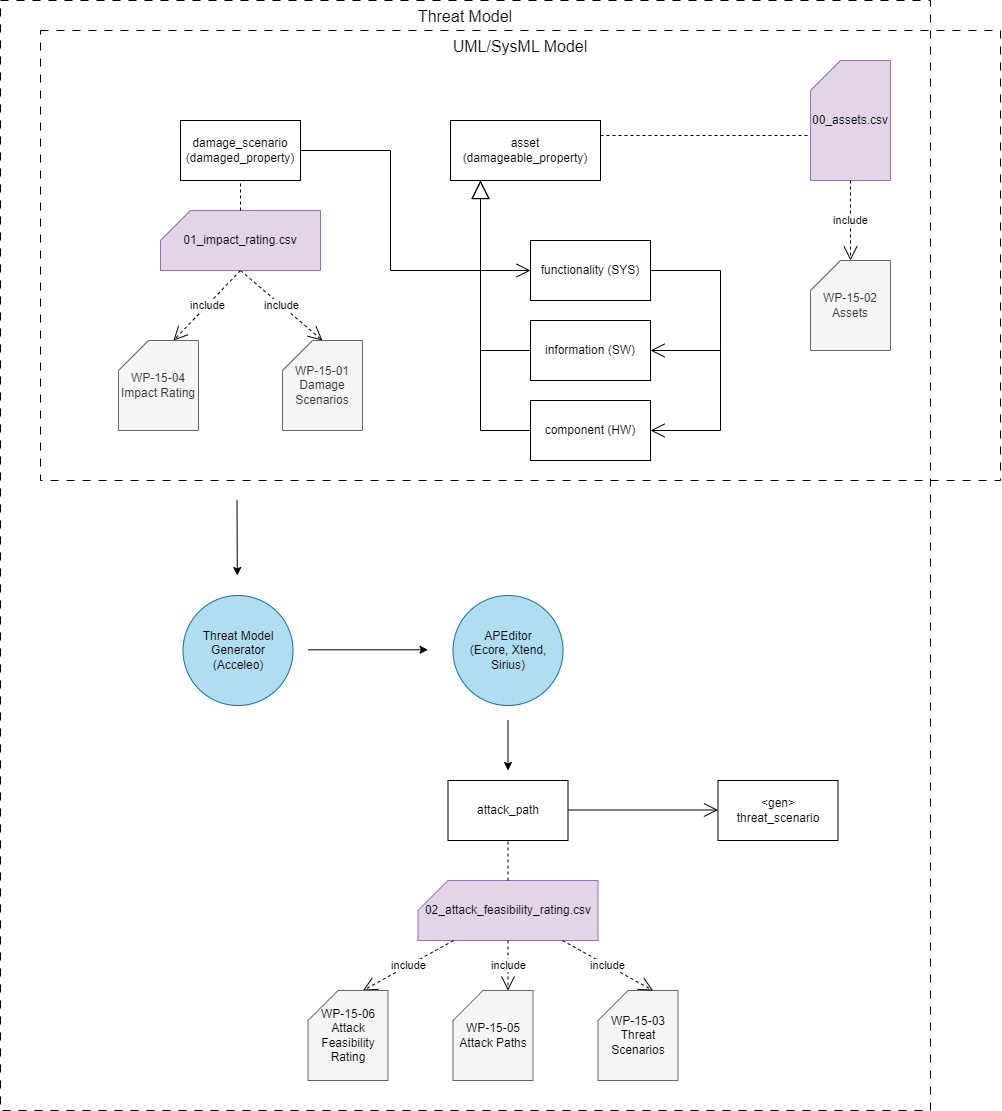
\includegraphics[width=130mm, keepaspectratio]{figures/05_overview.png}
	\caption{Megvalósítás áttekintése}
	\label{fig:05_OVERVIEW}
\end{figure}

Itt először kiemelném a fenyegetésmodell és a rendszermodell közös halmazában lévő tartalmakat. Ez a rendszermodell egy Papyrus projekt formájában készült el. Tartalmazza a \textit{Kihasználási eset diagramot} és a \textit{Termékleírást}. Ezek tartalmazzák az értékeket, funkcionalitást és a lehetséges károkozásokat, amelyekből két dokumentum állítható majd elő, amelyek három ISO 21434 workproduct-ot fednek. 

A következő elem a Threat Model Generator ami egy Acceleo script a Papyrus modellező eszközhöz integrálva és a cybersecurity profil alapján állít elő egy kezdeti modell fájlt amelyet a fenyegetésmodellező eszközzel fogunk tudni megnyitni.

A fenyegetésmodellező eszköz az APEditor (Attack Path Editor) amelyben lehetőségünk van a termékleírás és kihasználási diagram tartalmai közti dependenciák meghatározására, valamint támadási fák és fenyegetések automatikus származtatására.

A támadási fák elkészítése után fogjuk tudni a modellből származtatni a támadás megvalósíthatóság értékelés dokumentumot ami további három ISO 21434 workproduct-ot fed le.

\section{Kiberbiztonsági modell származtatása}

A kiberbiztonsági modell származtatása egy fontos lépése a kockázatelemzési folyamatnak. Előkészíti a fenyegetésmodellünket illetve teremt egyfajta nyomon követhetőséget a rendszermodell és a kiberbiztonsági modell között.

\subsection{Kiberbiztonsági profil}

A profilban négy sztereotípia került meghatározásra. Egyrészről a UseCase UML metaosztályát bővíti a damage\_scenario sztereotípia amellyel a károkozásokat tudjuk jelölni. A károkozásokhoz fel lett véve attribútumként, hogy azt mely kiberbiztonsági tulajdonság sérülése okozta.

A Component UML metaosztályt bőviti a functionality, component illetve az information sztereotípia. Itt a functionality jelenti a rendszerszintű funkcionalitást, ennek nincsenek az UML profilban attribútumai mivel azokat majd a kapcsolódó károkozások alapján fogjuk tudni meghatározni az elemzés későbbi fázisában. A component jelzi a HW komponenseket (pl. csatlakozó, modulok, áramkörök), az information pedig a SW szintű információkat (pl. szoftver, kriptográfiai adatok, üzenetek). Az utóbbi kettő az Asset (\textit{érték}) absztrakt osztályból van származtatva, ebből öröklik a kiberbiztonsági tulajdonságaikat.

\begin{figure}[!ht]
	\centering
	\includegraphics[width=130mm, keepaspectratio]{figures/05_Profile_Diagram.PNG}
	\caption{Kiberbiztonsági profil (UML)}
	\label{fig:05_UML_PROFILE}
\end{figure}

\subsection{Fenyegetésmodell generátor}

A fenyegetésmodell generátor egy Acceleo nyelven írt szkript, amelynek a feladata a Papyrus-ban szerkesztett .uml fájloknak a beolvasása és a tartalmuk alapján egy .apeditor fájlnak a generálása, amelyet a fenyegetésmodellező eszközben lehet tovább szerkeszteni.

A projekt felépítése és a dependenciák a \ref{fig:05_tmgen_arch} ábrán láthatóak.

\begin{figure}[!ht]
	\centering
	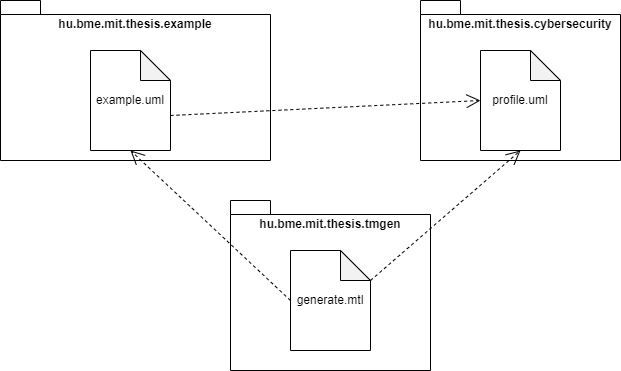
\includegraphics[width=130mm, keepaspectratio]{figures/05_package_tmgen.png}
	\caption{Threat Model Generator dependenciái}
	\label{fig:05_tmgen_arch}
\end{figure}

A \textbf{hu.bme.mit.thesis.example} projekt tartalmazza a kihasználási eset diagramot és a termékleírást, valamint applikálja a \textbf{hu.bme.mit.thesis.cybersecurity} projektben definiált kiberbiztonsági profil sztereotípiáit.

A \textbf{hu.bme.mit.thesis.tmgen} tartalmazza a \textbf{generate.mtl} fájlt ami egy Acceleo nyelven írt Model-To-Text generátor. Ez fogja előállítani a projekt \textit{generated} mappájába az \textbf{example.apeditor} fájlt, amelyet át lehet majd másolni a fenyegetésmodellező eszköz \textit{runtime} környezetében létrehozott projektekbe.

\section{Fenyegetésmodellező eszköz}

A fenyegetésmodellező eszköz teszi lehetővé a károkozások, funkcionalitások és értékek közti dependencia beállítását, a támadási fák szerkesztését, illetve a szabványos dokumentumok generálását.

Ennek a projektnek az áttekintése a \ref{fig:05_apeditor_arch} ábrán látható.

\begin{figure}[!ht]
	\centering
	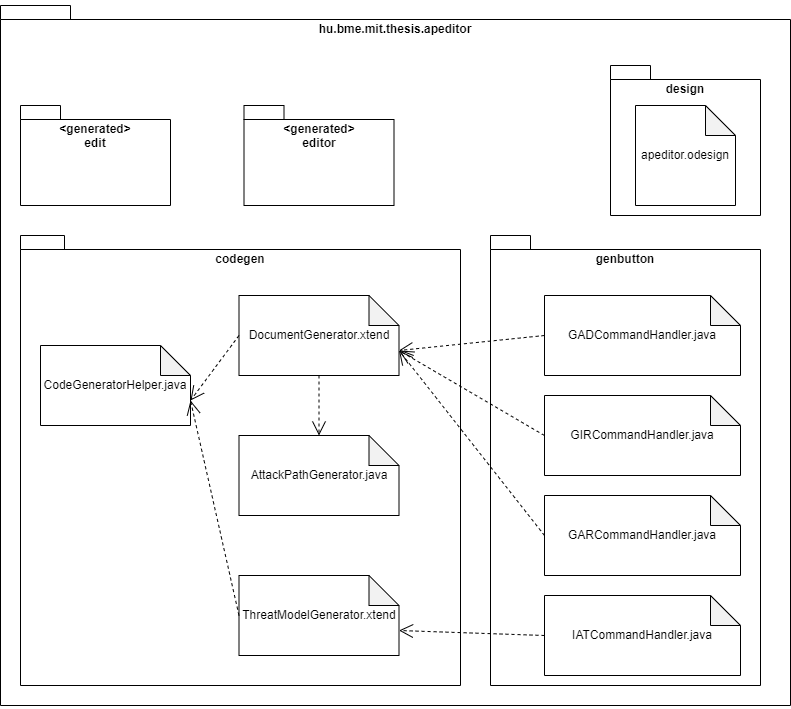
\includegraphics[width=130mm, keepaspectratio]{figures/05_package_apeditor.png}
	\caption{APEditor projekt felépítése és dependenciái}
	\label{fig:05_apeditor_arch}
\end{figure}

A \textbf{hu.bme.mit.thesis.apeditor} projektben található az \textit{apeditor.ecore} fájl ami a metamodellt tartalmazza, illetve az Eclipse Modelling Framework által generált fájlokat.

A \textbf{hu.bme.mit.thesis.apeditor.edit} illetve a \textbf{hu.bme.mit.thesis.apeditor.editor} projektek szintén az EMF által lettek generálva, ezek adják meg a modell szerkesztő felületének az alapjait.

A \textbf{hu.bme.mit.thesis.apeditor.design} tartalmaz egy Sirius keretrendszert használó \textit{apeditor.odesign} fájlt amely a támadási fáknak a grafikus megjelenítését és szerkesztő felületét írja le.

A \textbf{hu.bme.mit.thesis.apeditor.genbutton} tartalmazza a plugin.xml-t amelyben az APEditor felhasználói felületén megjelenítendő gombok vannak leírva, valamint a gombok megnyomásával futtatott .java fájl is itt kerül összelinkelésre. A négy .java fájl a különböző funkcionalitását definiálják.

\begin{itemize}
	\item \textbf{GADCommandHandler.java} Asset Definition workproduct generálását viszi véghez a \textbf{hu.bme.mit.thesis.apeditor.codegen} projektben definiált funkcionalitás aktiválásával
	\item \textbf{GIRCommandHandler.java} Impact Rating workproduct generálását viszi véghez a \textbf{hu.bme.mit.thesis.apeditor.codegen} projektben definiált funkcionalitás aktiválásával
	\item \textbf{GARCommandHandler.java} Attack Feasibility Rating workproduct generálását viszi véghez a \textbf{hu.bme.mit.thesis.apeditor.codegen} projektben definiált funkcionalitás aktiválásával
	\item \textbf{IATCommandHandler.java} Inicializálja a támadási fákat az \textbf{hu.bme.mit.thesis.apeditor.codegen} projektben definiált funkcionalitás aktiválásával
\end{itemize} 

Végül az \textbf{hu.bme.mit.thesis.apeditor.codegen} tartalmazza a kódgeneráláshoz szükséges osztályokat és függvényeket. Itt egyrészről a \textit{DocumentGenerator.xtend} fájl tartalmazza azokat az Xtend-ben megírt függvényeket, amelyek a szabványos workproduct-ok előállításához szükségesek, másrészről az Attack Feasibility Rating generálásakor, használja az \textit{AttackPathGenerator.java} függvényeit amelyek a támadási fákat fejti ki támadási útvonalakká amelyek támadási lépésekből állnak.

Az \textit{ThreatModelGenerator.xtend} a modellből generálja le a támadási fák kezdeti állapotát és aztán azokat írja bele a modellfájlba. Ezzel bővítve a szerkesztett modellt.

Mindkét Xtend fájl a \textit{CodeGeneratorHelper.java} fájlt használja még a fájlba író és fájlt olvasó műveletek elvégzésére.

\subsection{Metamodel}

\begin{figure}[!ht]
	\centering
	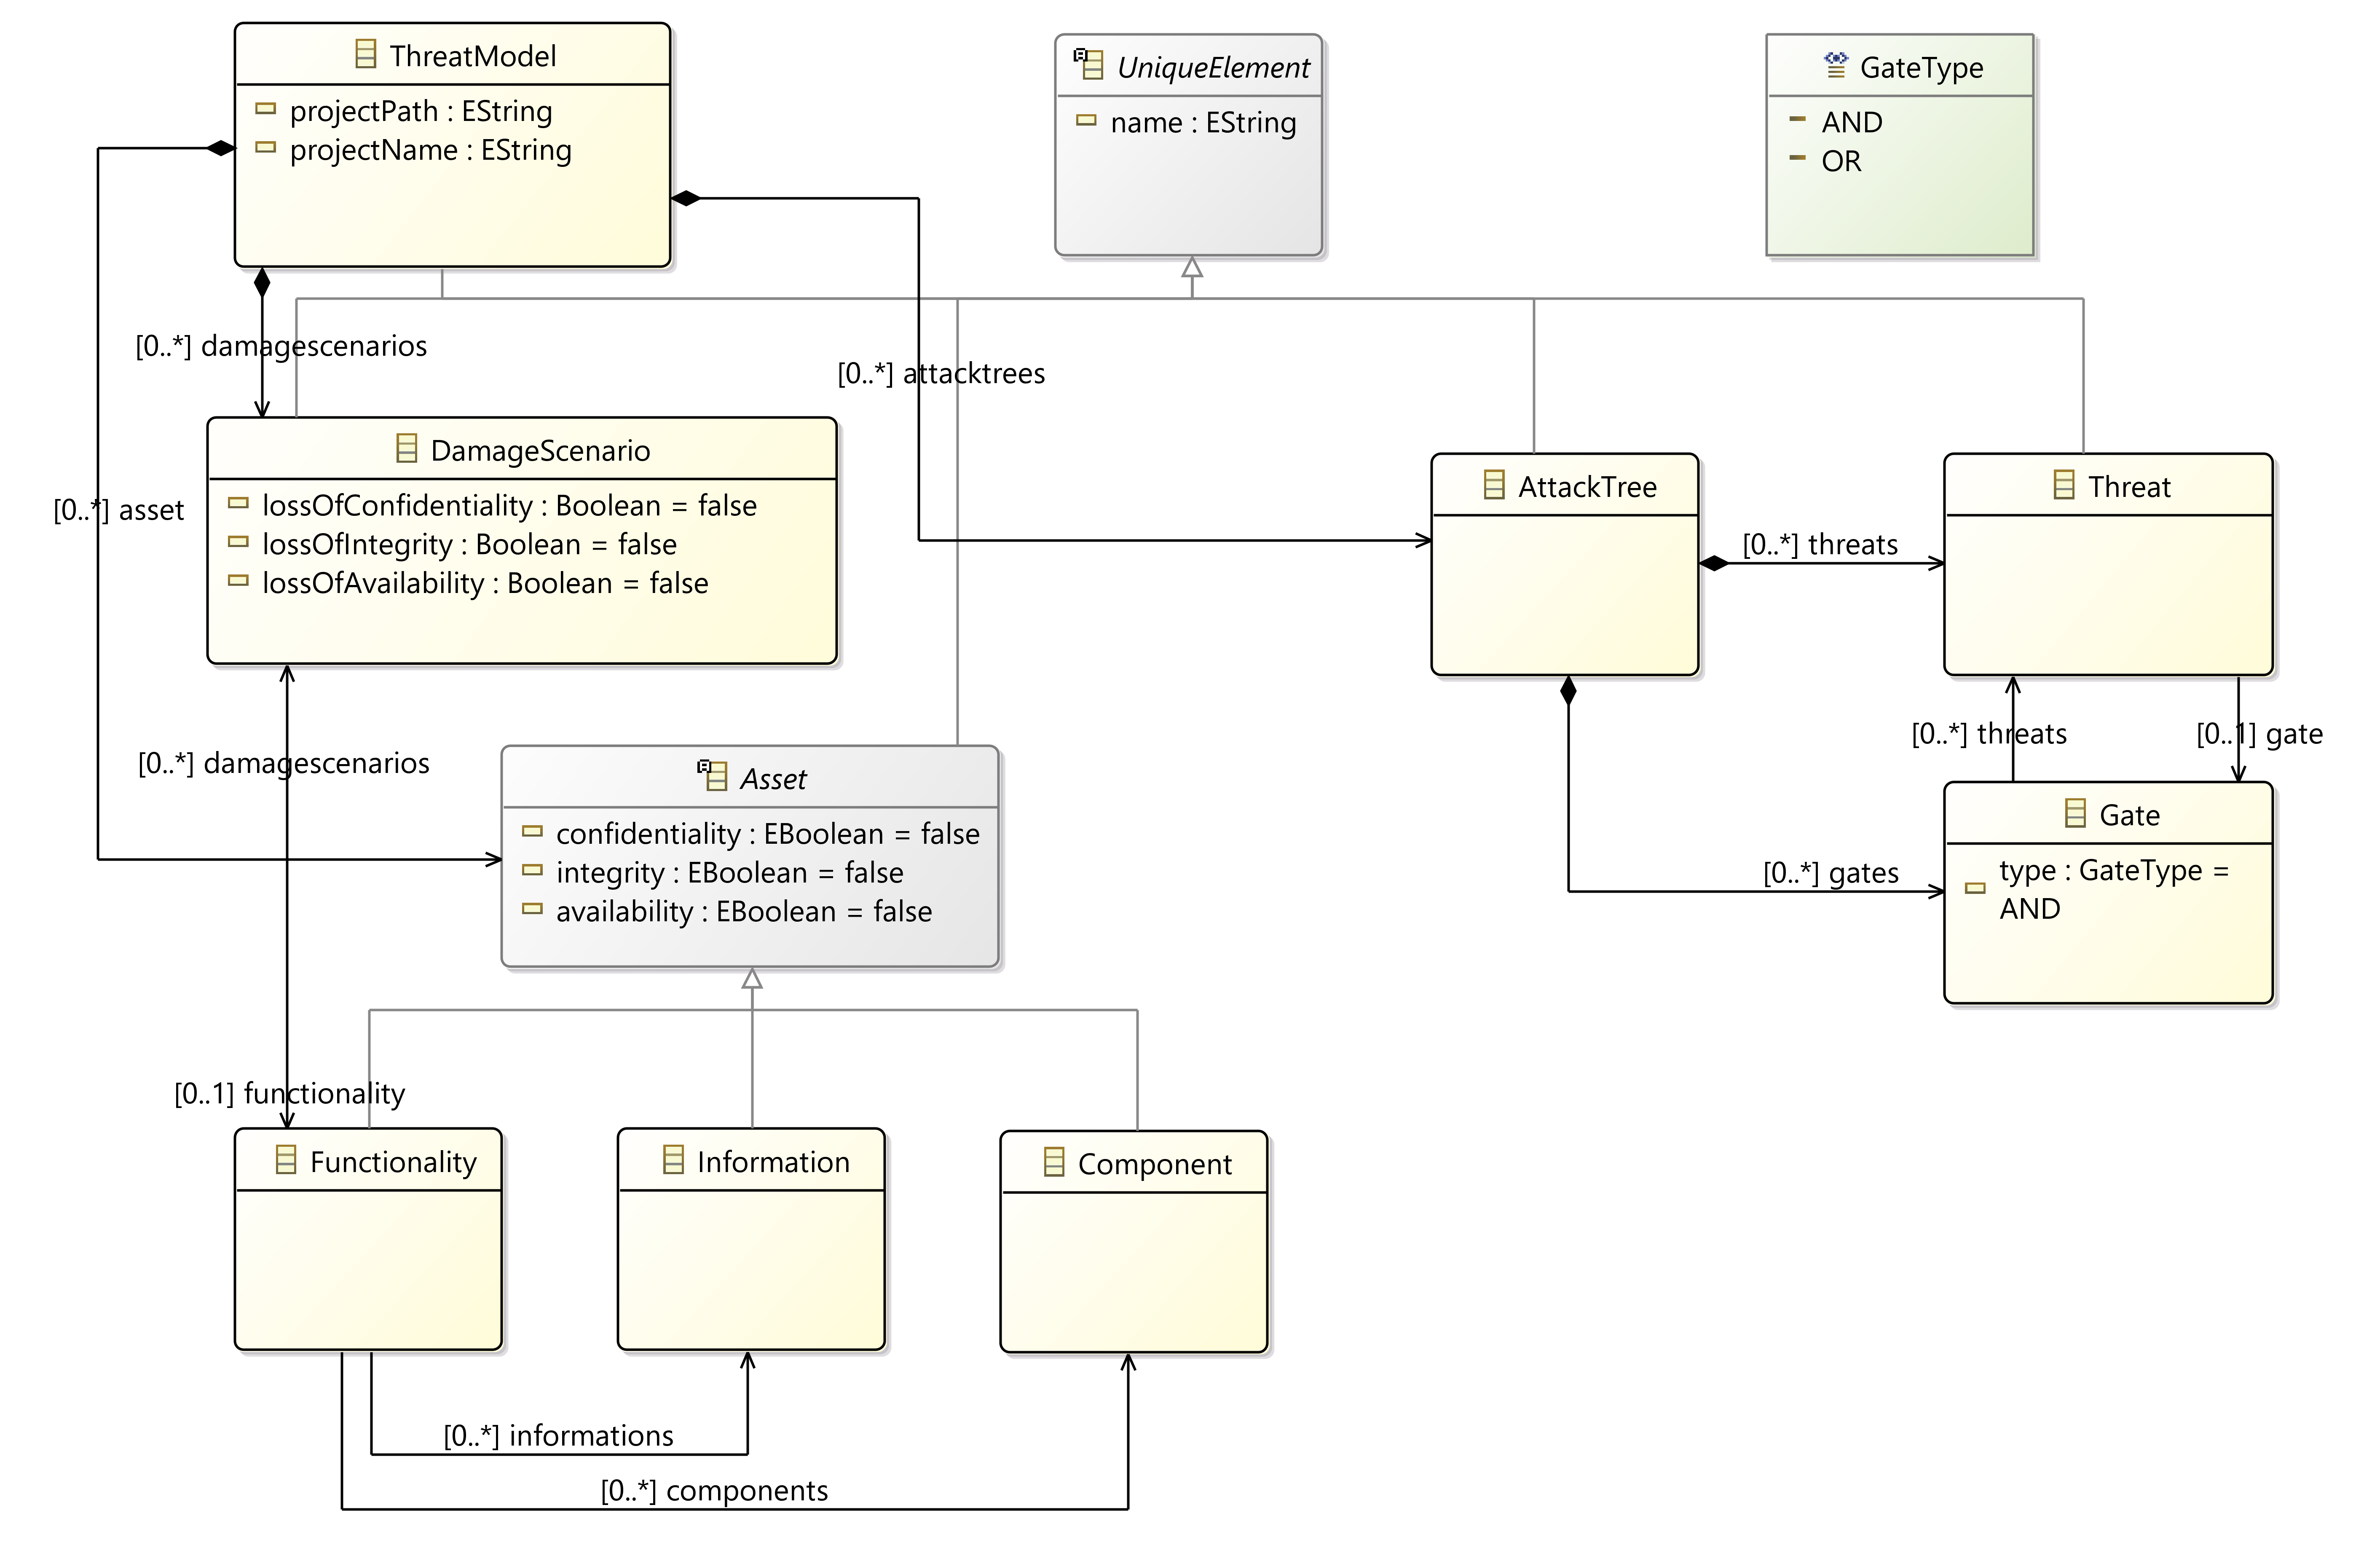
\includegraphics[width=130mm, keepaspectratio]{figures/05_metamodel.png}
	\caption{apeditor.ecore fájlban definiált metamodell}
	\label{fig:05_metamodel}
\end{figure}

A metamodell az ISO 21434 szabványban definiált különböző elemeket és megnevezéseket használja. Az elemzésben felhasznált elemek között a szabvány alapján határoztam meg a kapcsolati függőségeket és ezeket tartalmazza a \textit{ThreatModel} objektum.

Az előzetes fenyegetésmodell származtatása fogja előállítani a \textbf{DamageScenario} és \textbf{Asset} listákat amelyeket fel is vesz a modellből generált \textbf{ThreatModel} objektum alá.

A generált modellben minden \textbf{DamageScenario} összerendelhető lesz egy \textbf{Functionality}-vel, ez a rendszerszintű \textbf{Asset}.

A dependenciákat a szintén generált \textbf{Information} (SW-szintű érték) és \textbf{Component} (HW-szintű érték) objektumoknak a \textbf{Functionality}-hez való rendelésével tettem lehetővé.

A támadási fáknak az inicializálása egy egy \textbf{AttackTree} létrehozásával történik az egyes \textbf{DamageScenario}-khoz. A \textbf{Threat}-ek az alapján vannak generálva, hogy a \textbf{DamageScenario}-hoz tartozó \textbf{Asset}-ek milyen kiberbiztonsági tulajdonságokkal rendelkeznek. A \textbf{Gate} objektumok pedig manuálisan kerülnek létrehozásra a támadási fa szerkesztő felületen.

Továbbá a \textbf{GateType} enumeráció teszi lehetővé a kapuk, a \textbf{UniqueElement} pedig az összes egyedi elem megkülönböztetését.

A \textbf{ThreatModel} rendelkezik egy projectPath és projectName property-vel, ezeket az értékeket a dokumentumok generálásához használjuk.


\subsection{Fenyegetésmodell szerkesztő felület}

A fenyegetésmodell szerkesztő felülete szolgál arra, hogy a dependenciákat meghatározza a SW- és HW-szintű értékek, valamint a funkcionalitás között, illetve, hogy allokáljuk a károkozásokhoz a funkcionalitást.

Ez a felület az Ecore modellből Eclipse Modelling Framework segítségével kerül generálásra. Megtekinthető a \ref{fig:05_tmeditor}

\begin{figure}[!ht]
	\centering
	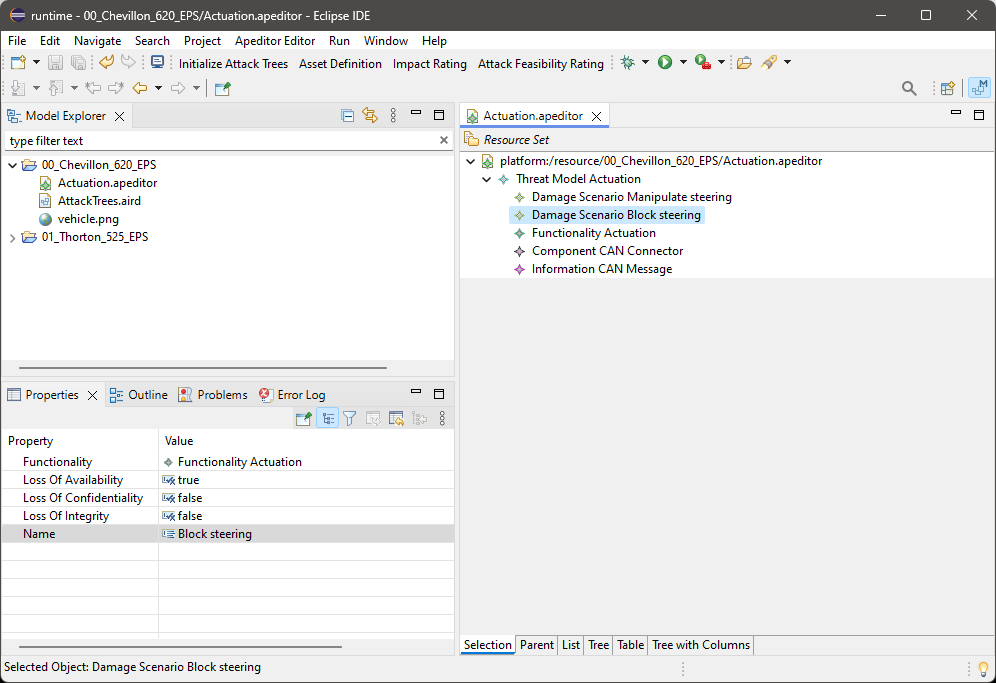
\includegraphics[width=130mm, keepaspectratio]{figures/05_tmeditor_ds.png}
	\caption{Fenyegetésmodell szerkesztő felület}
	\label{fig:05_tmeditor}
\end{figure}

Az ábrán látható a Model Explorer-ben az éppen megnyitott projekt, valamint az abban lévő fenyegetésmodellek a .apeditor fájlkiterjesztésekkel, illetve a támadási fa diagramok lesznek láthatóak a .aird fájl megnyitásával.

A jobb oldalon lehet böngészni és felvenni új elemeket a fenyegetésmodellbe, illetve itt kell kiválasztani a szerkesztendő elemet.

Bal alul pedig a properties fülnél látjuk a metamodellben definiált attribútumokat és szerkeszthetjük a felvett értékeket (value).

\subsection{Támadási fák inicializálása}

A fenyegetésmodell kiválasztásával, a projekt útvonal és nevek beállítását követően el is végezhetjük a támadási fák inicializálását az \ref{fig:05_at_init} ábrán látható gomb megnyomásával.

\begin{figure}[!ht]
	\centering
	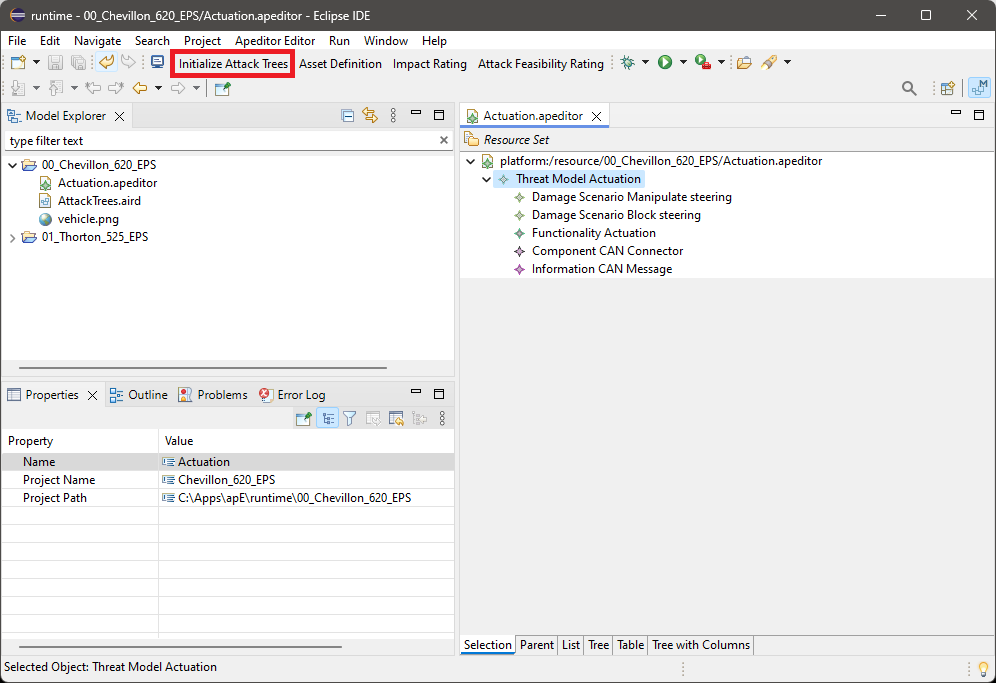
\includegraphics[width=130mm, keepaspectratio]{figures/05_tmeditor.png}
	\caption{Támadási fák inicializálását végző kiterjesztés}
	\label{fig:05_at_init}
\end{figure}

Ez a kiterjesztés fogja használni a kódgenerátor plugin \textbf{ThreatModelGenerator.xtend} osztályában implementált funkcionalitást meghívni, amely a projekt útvonalon található fenyegetésmodell fájlt feltölti a tartalma alapján előálló támadási fákkal. Az inicializálás eredménye a \ref{fig:05_at_inited} ábrán látható.

\begin{figure}[!ht]
	\centering
	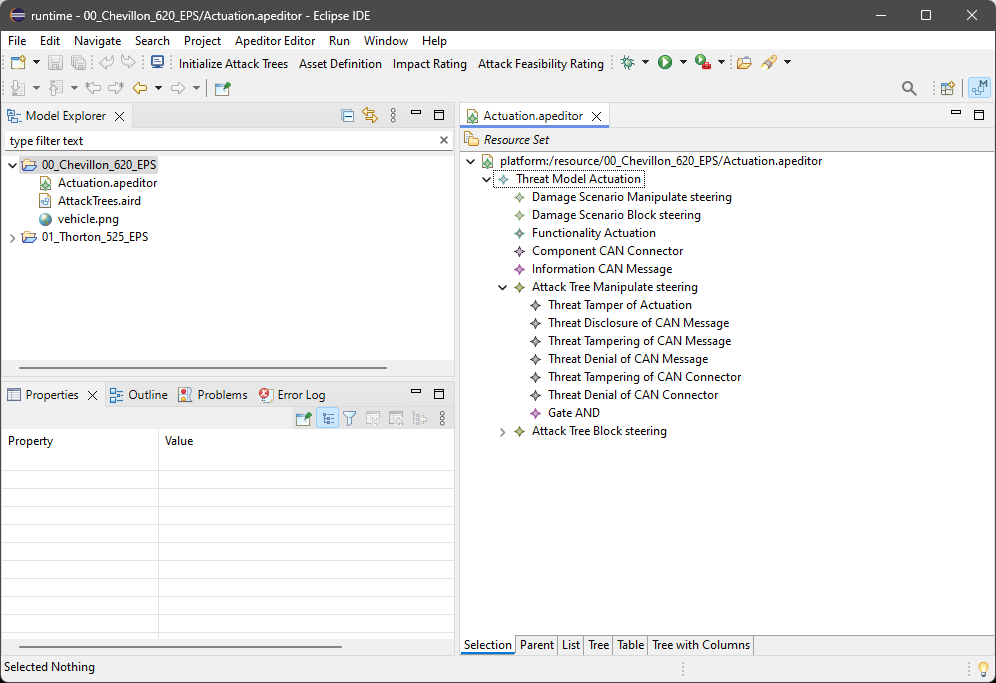
\includegraphics[width=130mm, keepaspectratio]{figures/05_at_inited.png}
	\caption{Támadási fák inicializálásának eredménye}
	\label{fig:05_at_inited}
\end{figure}

\subsection{Támadási fa szerkesztő felület}

A szerkesztő felületet az Eclipse Sirius keretrendszerére alapozva készítettem el. A projektben létrehozott .aird fájlra kattintva lehet a támadási fákhoz új reprezentációt létrehozni, ennek az eredménye a \ref{fig:05_at_editor_1} ábrán látható.

\begin{figure}[!ht]
	\centering
	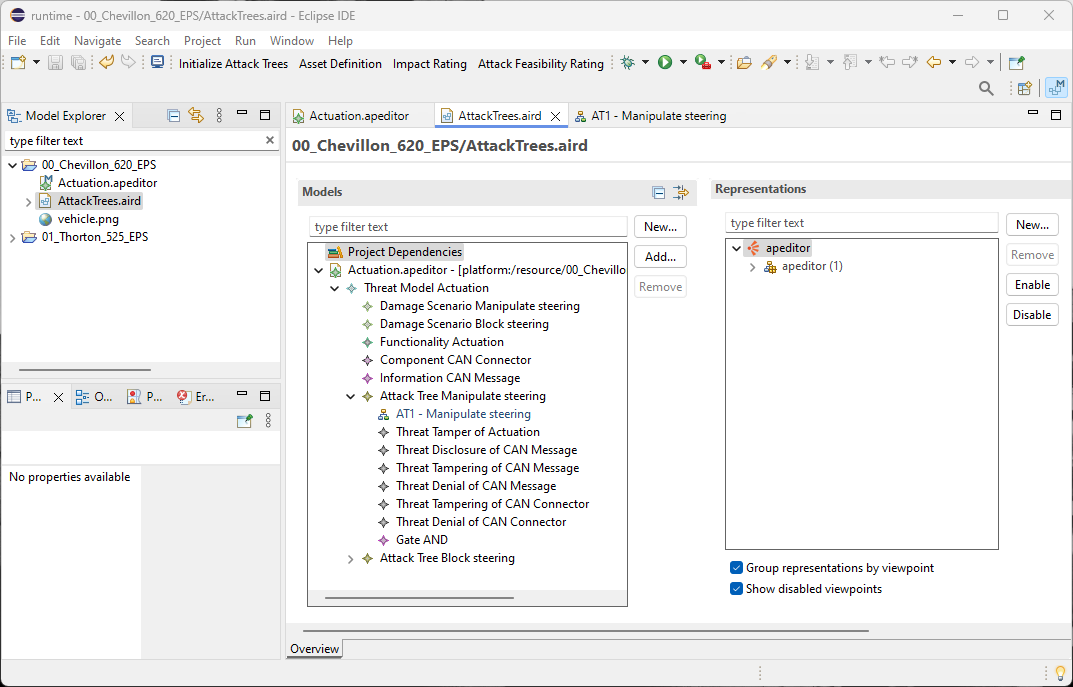
\includegraphics[width=130mm, keepaspectratio]{figures/05_ateditor_1.png}
	\caption{Reprezentáció létrehozása}
	\label{fig:05_at_editor_1}
\end{figure}

A létrehozás automatikusan meg is fogja nyitni a szerkesztőfelületet (\ref{fig:05_ateditor_2} ábra) amelyen megfigyelhető a gyökér elemhez automatikusan létrehozott első kapu, amelynek típusa a properties fülön állítható.

\begin{figure}[!ht]
	\centering
	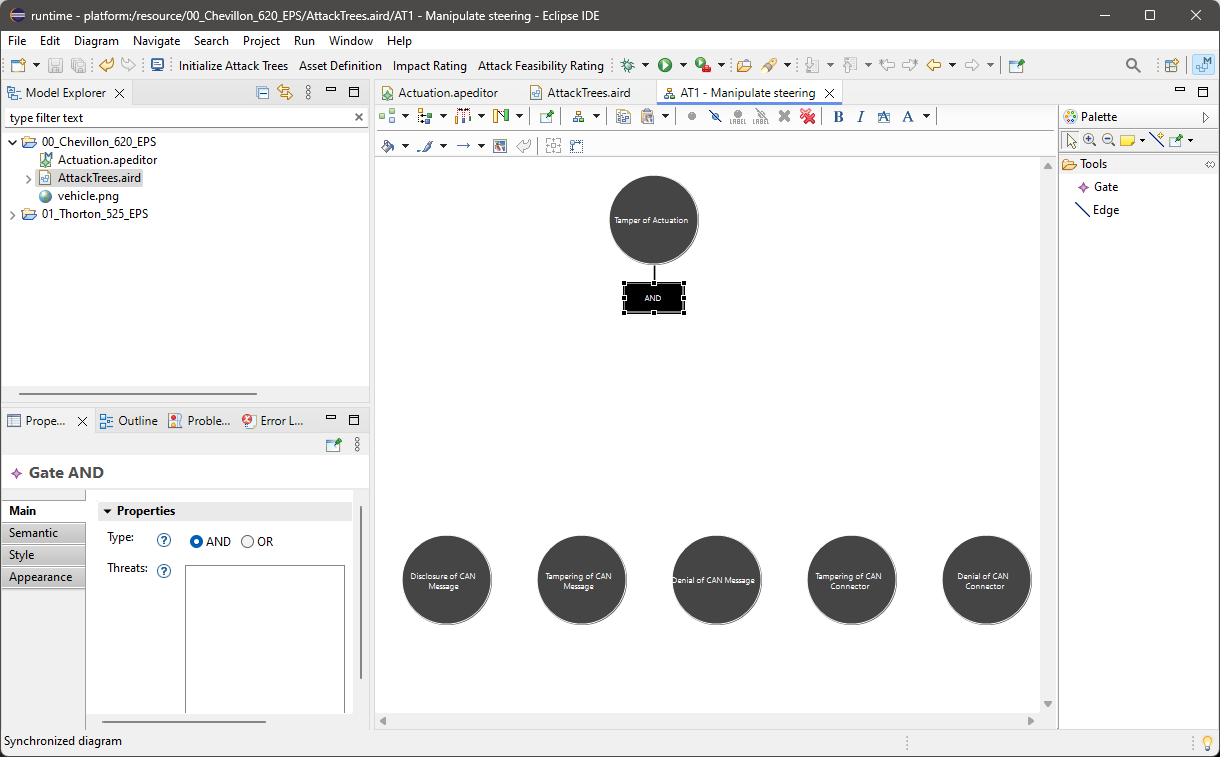
\includegraphics[width=130mm, keepaspectratio]{figures/05_ateditor_2.png}
	\caption{Támadási fa szerkesztő felület (kezdeti)}
	\label{fig:05_ateditor_2}
\end{figure}

A jobb oldalt a Tools menü alatt találhatóak az új modellelemek létrehozásához szükséges eszközök. Potenciálisan vagy új kapukat fogunk létrehozni vagy a kapuk bemenetére kötünk fenyegetéseket. Szintén itt van lehetőség törölni olyan fenyegetéseket amelyek nem relevánsak a támadási fához. Egy kész hibafa megtekinthető a \ref{fig:05_ateditor_3} ábrán.

\begin{figure}[!ht]
	\centering
	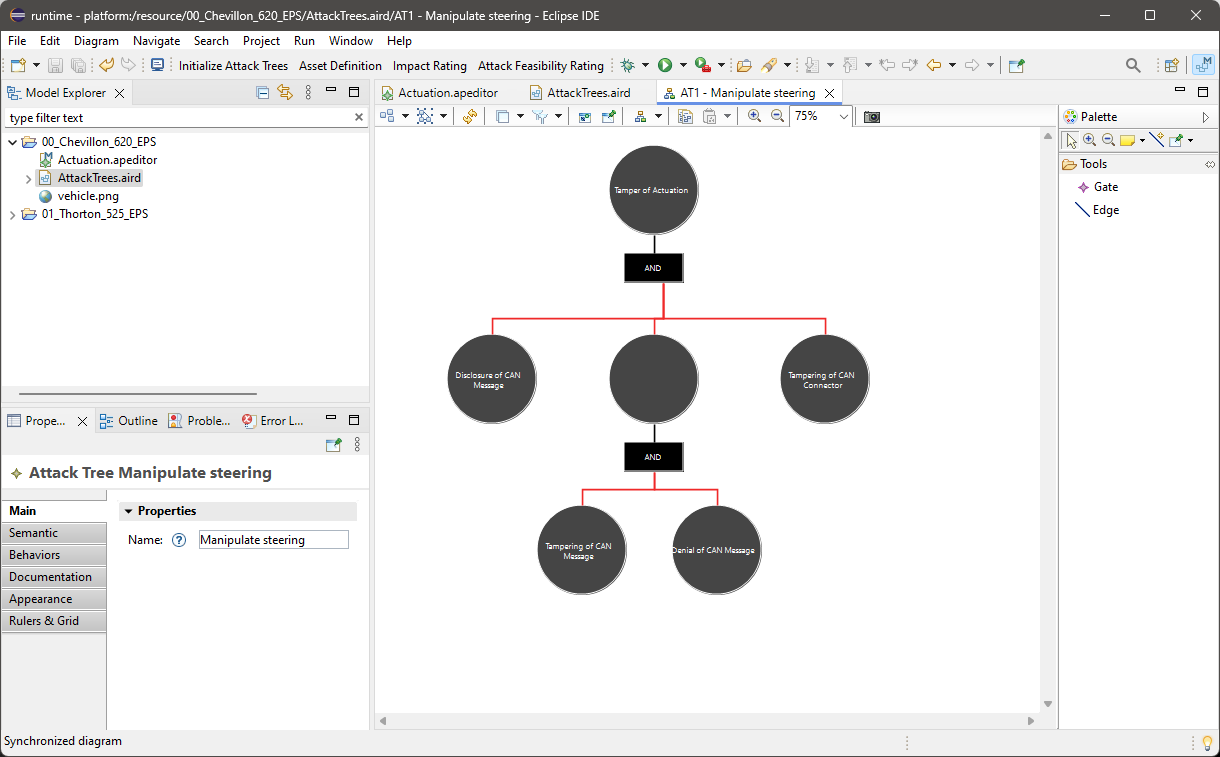
\includegraphics[width=130mm, keepaspectratio]{figures/05_ateditor_3.png}
	\caption{Támadási fa szerkesztő felület (befejezett)}
	\label{fig:05_ateditor_3}
\end{figure}

A Sirius leírófájl benne a grafikusan megjelenítendő elemekkel pedig a \ref{fig:05_ateditor_4} ábrán látható.

\begin{figure}[!ht]
	\centering
	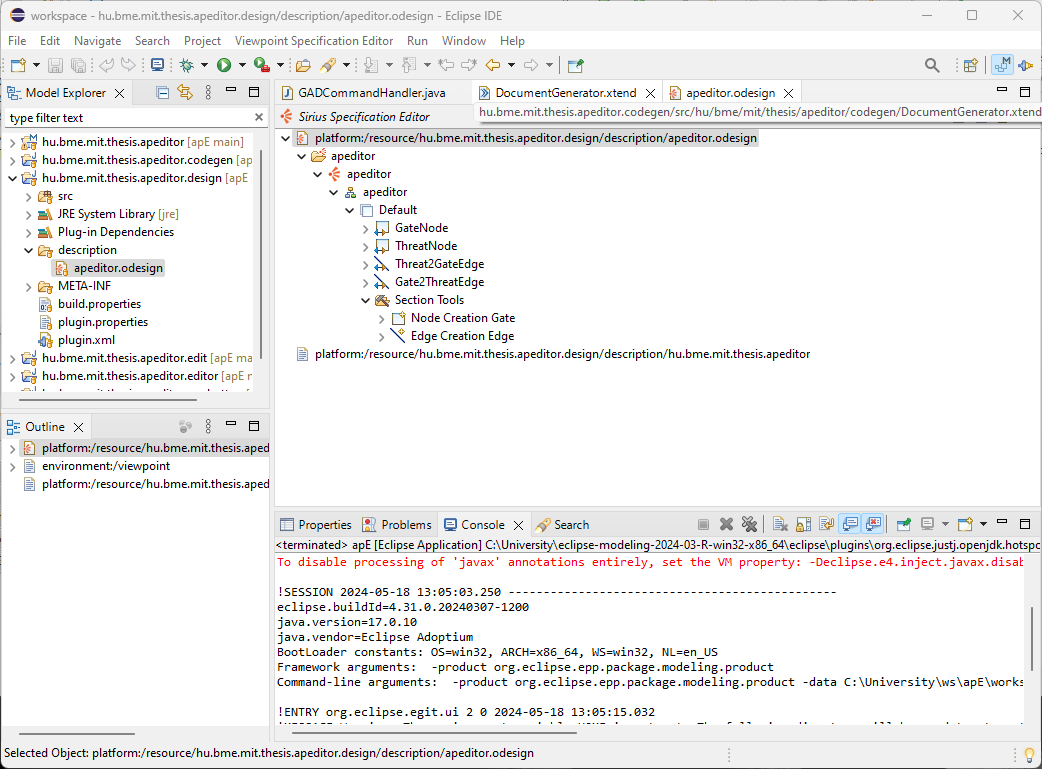
\includegraphics[width=130mm, keepaspectratio]{figures/05_ateditor_4.png}
	\caption{Támadási fa szerkesztő leírófájlja}
	\label{fig:05_ateditor_4}
\end{figure}

\subsection{Dokumentum generátor}

A dokumentumgenerálást szintén egy plugin-ként definiált gomb megnyomásával lehet elvégezni, miután a mérnök kiválaszotta a fenyegetésmodellt és beállította helyesen a projekt útvonalat és neveket.

\begin{figure}[!ht]
	\centering
	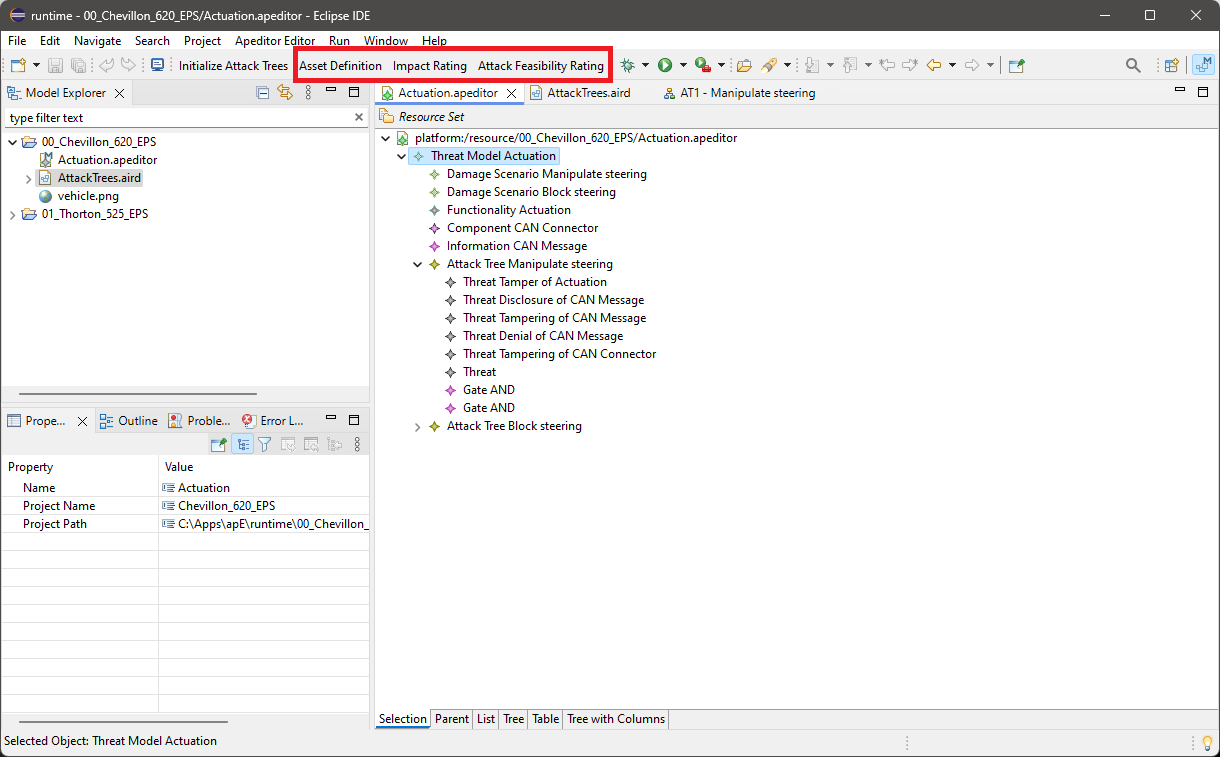
\includegraphics[width=130mm, keepaspectratio]{figures/05_docgen_1.png}
	\caption{Dokumentumok generálását végző kiterjesztés}
\end{figure}

A generálás elvégzése után a projekt alatt megjelennek a manuális analízis elvégzéséhez használható .csv fájlok.

\begin{figure}[!ht]
	\centering
	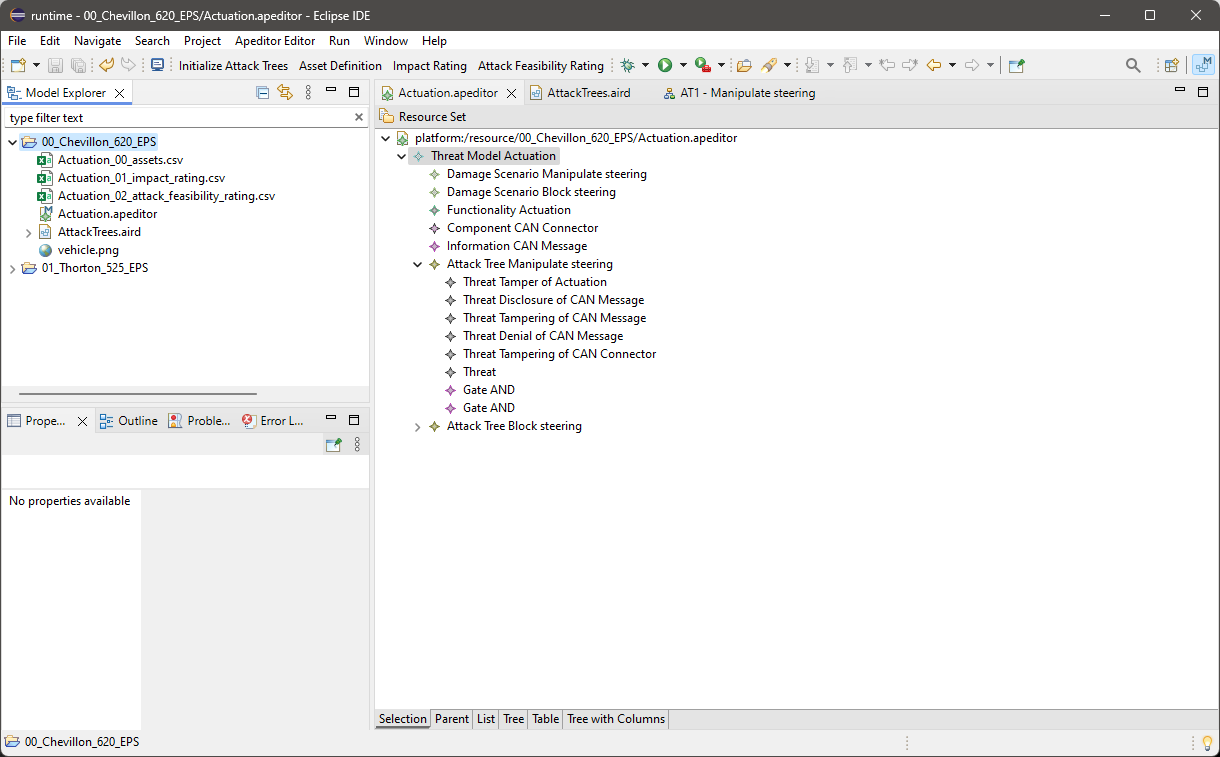
\includegraphics[width=130mm, keepaspectratio]{figures/05_docgen_2.png}
	\caption{Generált dokumentumok}
\end{figure}
